% chktex-file 13
\chapter{MODELAGEM LÓGICA}
Este capítulo apresenta a modelagem lógica do sistema de gerenciamento 
de comissões artísticas por meio de fluxogramas. As ilustrações detalham 
a jornada do usuário.
\section{Fluxo de Navegação e Interface Inicial}
A estrutura lógica da aplicação é iniciada por um menu de navegação, 
conforme ilustrado na Figura~\ref{fig:fluxo_inicio}.
\section{Gestão de Clientes e Pedidos}
\subsection{Cadastro de Clientes}
A Figura~\ref{fig:fluxo_cliente} especifica os dados necessários para 
realizar o cadastro de clientes.
\subsection{Abertura de Pedidos}
O processo de criação de pedido (Figura~\ref{fig:fluxo_pedido}) atrela 
um cliente cadastrado aos dados de sua solicitação.
\section{Consulta e Manutenção de Dados}
\subsection{Consulta e Baixa de Pedidos}
A visualização de pedidos (Figura~\ref{fig:fluxo_consulta}) demonstra as 
opções de gerenciamento.
\subsection{Edição e Atualização do pedido}
O fluxo de edição (Figura~\ref{fig:fluxo_edicao}) detalha as atualizações 
possíveis em um pedido existente.
\subsection{Edição e atualização de dados do cliente}
O fluxo de edição (Figura~\ref{fig:fluxo_edicao_cliente}) detalha as 
atualizações possíveis nos dados cadastrais de um cliente.
\clearpage
\begin{figure}[htbp]
    \centering
    \caption{Fluxograma da Interface Inicial}\label{fig:fluxo_inicio}
    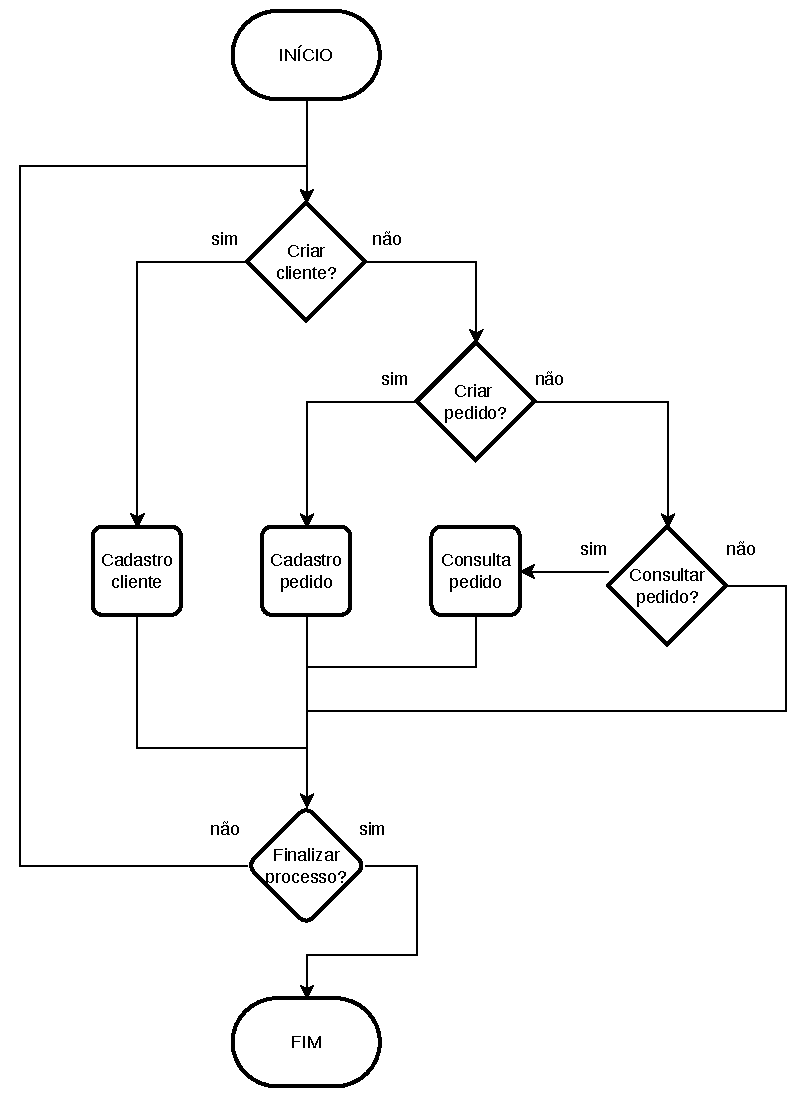
\includegraphics[height=0.75\textheight, keepaspectratio]
    {caps/imagens/TelaInicial.pdf}
    \fonte{Elaborado pelos autores (2026).}
\end{figure}
A figura demonstra as funções da aplicação, voltada ao usuário que organiza 
os pedidos de seus clientes, possibilitando o cadastro de clientes, a criação 
de pedidos e a consulta dos mesmos.
\clearpage
\begin{figure}[htbp]
    \centering
    \caption{Fluxograma do Processo de Cadastro de Cliente}\label{fig:fluxo_cliente}
    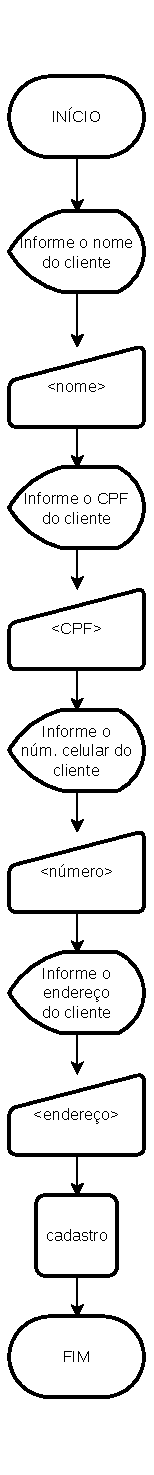
\includegraphics[height=0.75\textheight, keepaspectratio]
    {caps/imagens/CadastroDeClientes.pdf}
    \fonte{Elaborado pelos autores (2026).}
\end{figure}
A figura especifica os dados necessários para realizar o cadastro de clientes 
a serem armazenados no banco de dados da aplicação.
\clearpage
\begin{figure}[htbp]
    \centering
    \caption{Fluxograma de Cadastro de Pedido}\label{fig:fluxo_pedido}
    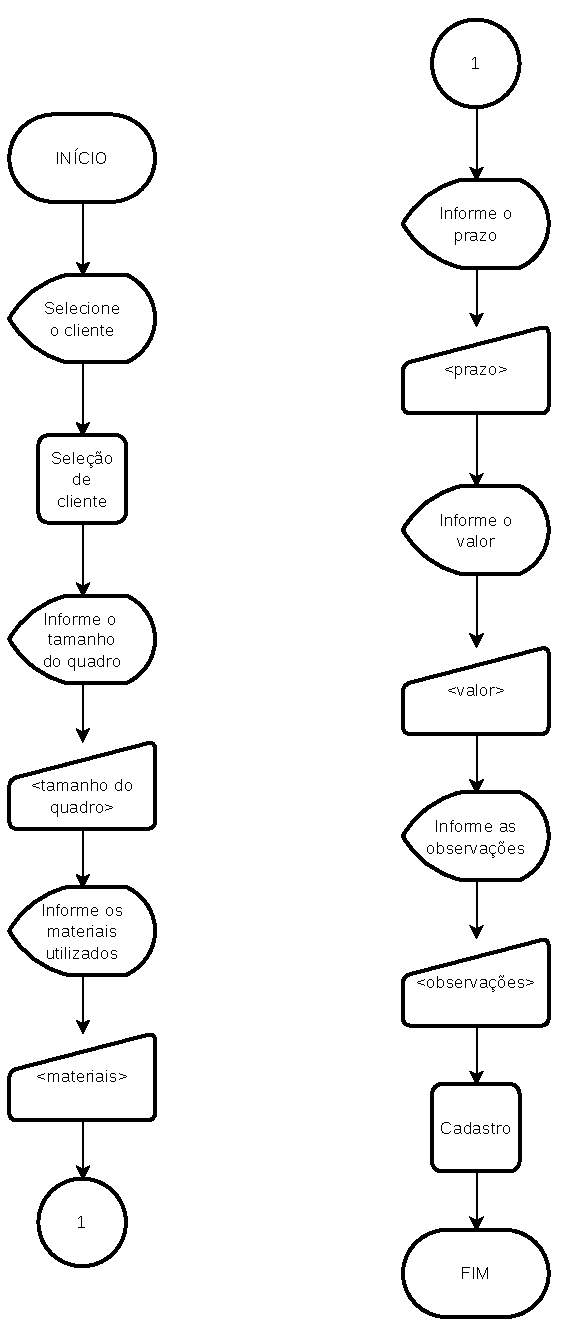
\includegraphics[height=0.75\textheight, keepaspectratio]
    {caps/imagens/CadastroDePedidos.pdf}
    \fonte{Elaborado pelos autores (2026).}
\end{figure}
A figura mostra o processo de criação de pedido, atrelando um cliente já 
cadastrado na aplicação aos dados específicos de sua solicitação.
\clearpage
\begin{figure}[htbp]
    \centering
    \caption{Fluxograma de Consulta de Pedidos}\label{fig:fluxo_consulta}
    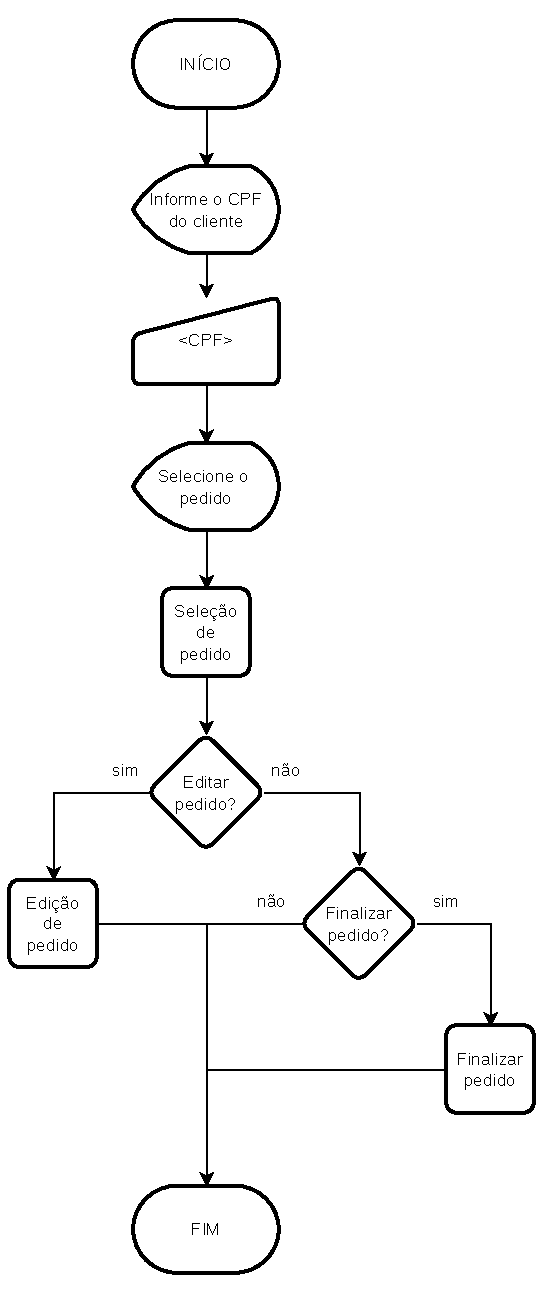
\includegraphics[height=0.75\textheight, keepaspectratio]
    {caps/imagens/ConsultaDePedidos.pdf}
    \fonte{Elaborado pelos autores (2026).}
\end{figure}
A figura demonstra as opções ao realizar a visualização de pedidos já 
cadastrados na aplicação, podendo alterar certas informações do pedido 
ou dar baixa em pedidos que já tenham sido concluídos pelo usuário.
\clearpage
\begin{figure}[htbp]
    \centering
    \caption{Fluxograma de Edição de Pedido}\label{fig:fluxo_edicao}
    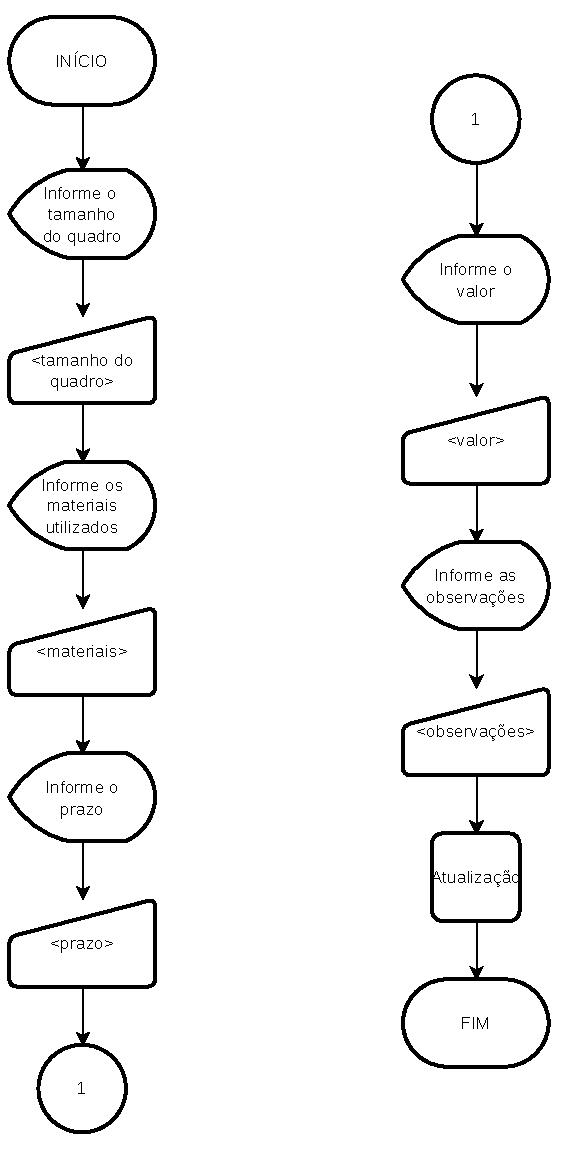
\includegraphics[height=0.75\textheight, keepaspectratio]
    {caps/imagens/AtualizacaoDePedidos.pdf}
    \fonte{Elaborado pelos autores (2026).}
\end{figure}
A figura mostra as possíveis edições que podem ser realizadas ao atualizar 
um pedido já cadastrado na aplicação.
\clearpage
\begin{figure}[htbp]
    \centering
    \caption{Fluxograma de Edição de Dados do Cliente}\label{fig:fluxo_edicao_cliente}
    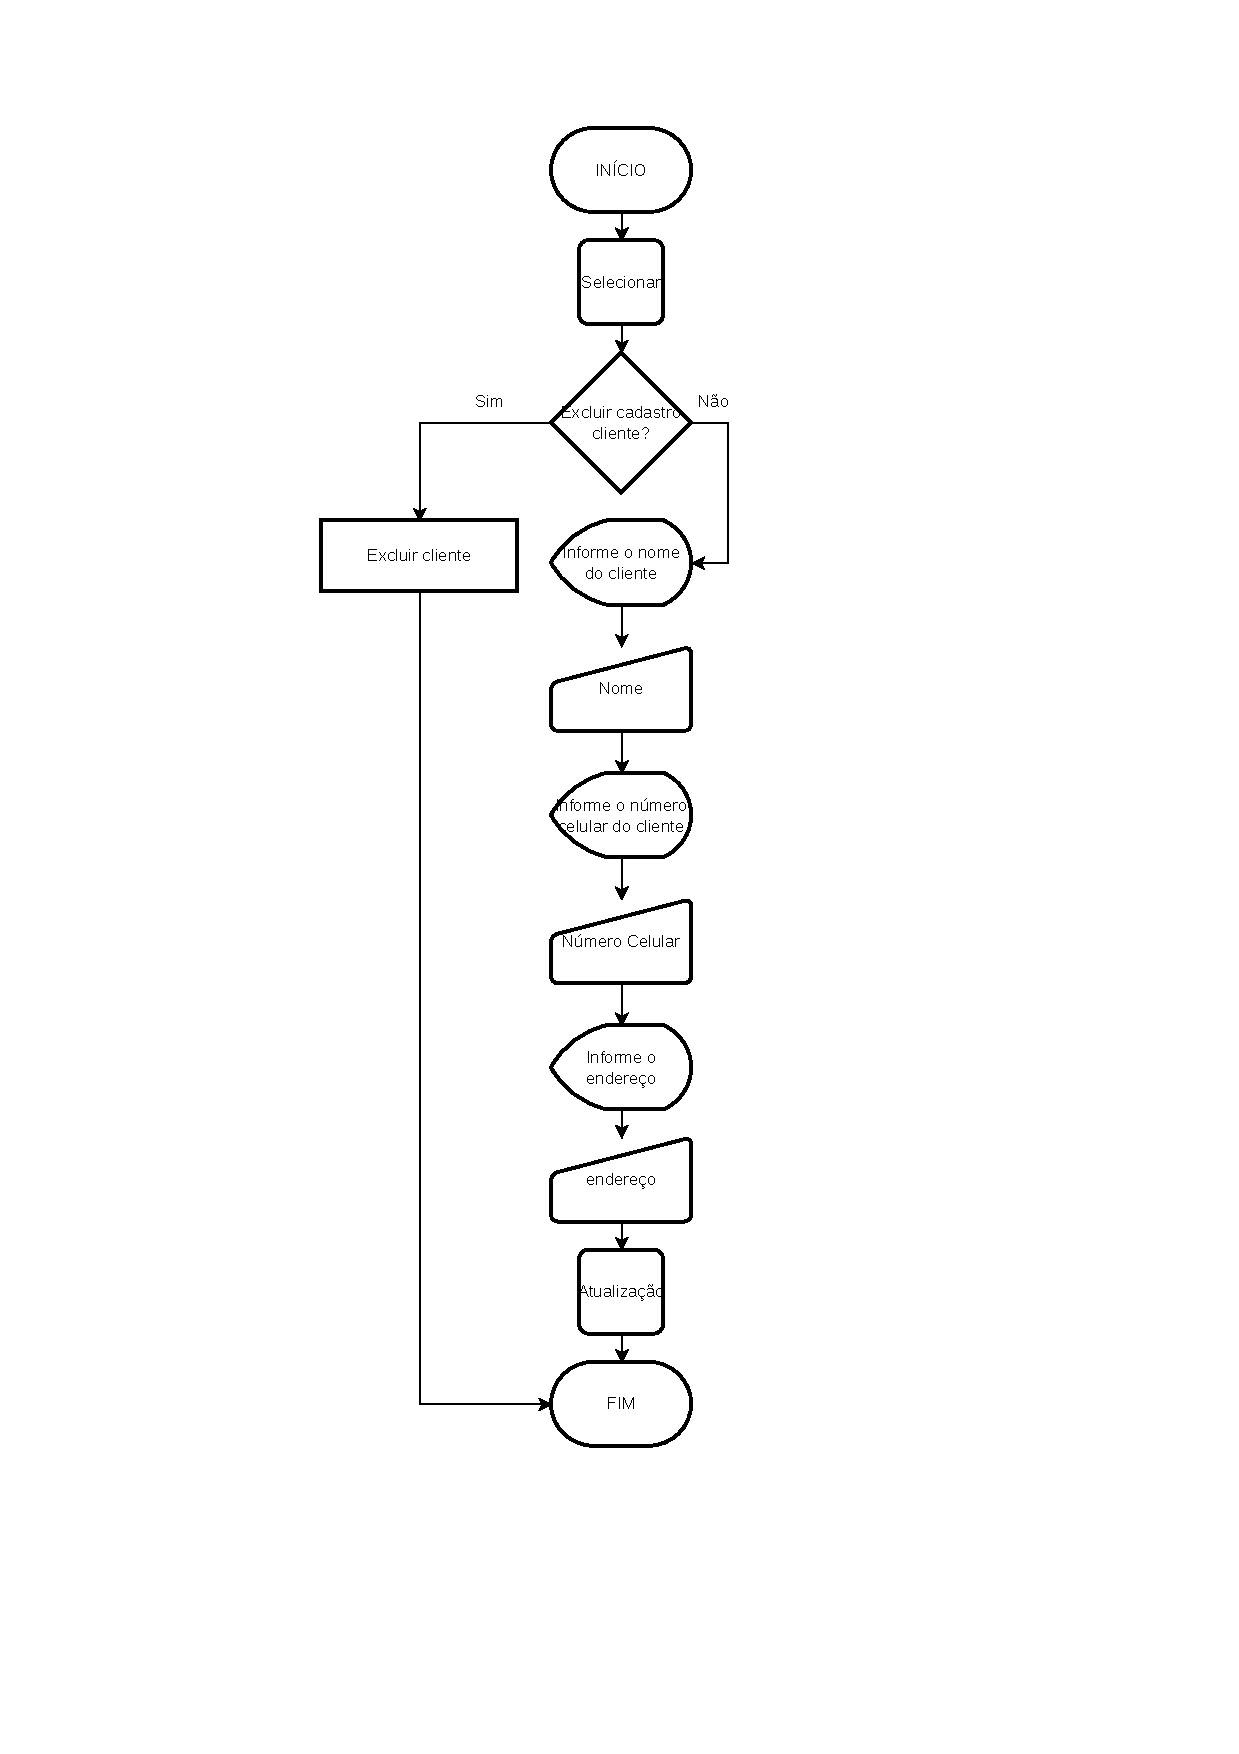
\includegraphics[height=0.75\textheight, keepaspectratio]
    {caps/imagens/EdicaoCliente.pdf}
    \fonte{Elaborado pelos autores (2026).}
\end{figure}
A figura mostra as possíveis edições que podem ser realizadas ao atualizar os 
dados cadastrais de um cliente.